\PassOptionsToPackage{unicode=true}{hyperref} % options for packages loaded elsewhere
\PassOptionsToPackage{hyphens}{url}
%
\documentclass[]{article}
\usepackage{lmodern}
\usepackage{amssymb,amsmath}
\usepackage{ifxetex,ifluatex}
\usepackage{fixltx2e} % provides \textsubscript
\ifnum 0\ifxetex 1\fi\ifluatex 1\fi=0 % if pdftex
  \usepackage[T1]{fontenc}
  \usepackage[utf8]{inputenc}
  \usepackage{textcomp} % provides euro and other symbols
\else % if luatex or xelatex
  \usepackage{unicode-math}
  \defaultfontfeatures{Ligatures=TeX,Scale=MatchLowercase}
\fi
% use upquote if available, for straight quotes in verbatim environments
\IfFileExists{upquote.sty}{\usepackage{upquote}}{}
% use microtype if available
\IfFileExists{microtype.sty}{%
\usepackage[]{microtype}
\UseMicrotypeSet[protrusion]{basicmath} % disable protrusion for tt fonts
}{}
\IfFileExists{parskip.sty}{%
\usepackage{parskip}
}{% else
\setlength{\parindent}{0pt}
\setlength{\parskip}{6pt plus 2pt minus 1pt}
}
\usepackage{hyperref}
\hypersetup{
            pdftitle={SDS 291 - Multiple Regression},
            pdfborder={0 0 0},
            breaklinks=true}
\urlstyle{same}  % don't use monospace font for urls
\usepackage[margin=1in]{geometry}
\usepackage{graphicx,grffile}
\makeatletter
\def\maxwidth{\ifdim\Gin@nat@width>\linewidth\linewidth\else\Gin@nat@width\fi}
\def\maxheight{\ifdim\Gin@nat@height>\textheight\textheight\else\Gin@nat@height\fi}
\makeatother
% Scale images if necessary, so that they will not overflow the page
% margins by default, and it is still possible to overwrite the defaults
% using explicit options in \includegraphics[width, height, ...]{}
\setkeys{Gin}{width=\maxwidth,height=\maxheight,keepaspectratio}
\setlength{\emergencystretch}{3em}  % prevent overfull lines
\providecommand{\tightlist}{%
  \setlength{\itemsep}{0pt}\setlength{\parskip}{0pt}}
\setcounter{secnumdepth}{0}
% Redefines (sub)paragraphs to behave more like sections
\ifx\paragraph\undefined\else
\let\oldparagraph\paragraph
\renewcommand{\paragraph}[1]{\oldparagraph{#1}\mbox{}}
\fi
\ifx\subparagraph\undefined\else
\let\oldsubparagraph\subparagraph
\renewcommand{\subparagraph}[1]{\oldsubparagraph{#1}\mbox{}}
\fi

% set default figure placement to htbp
\makeatletter
\def\fps@figure{htbp}
\makeatother


\title{SDS 291 - Multiple Regression}
\author{}
\date{\vspace{-2.5em}January 27, 2020}

\begin{document}
\maketitle

\hypertarget{lecture-notes}{%
\section{Lecture Notes}\label{lecture-notes}}

Here is some space to take notes on the slides we'll go through in class
with some prompts for key ideas to pay attention to.

\begin{itemize}
\tightlist
\item
  \textbf{Sample, Population, Statistics, Parameters}
\end{itemize}

\vspace{0.5in}

\begin{itemize}
\tightlist
\item
  \textbf{Types of Variables}
\end{itemize}

\vspace{1.5in}

\begin{itemize}
\tightlist
\item
  \textbf{Describing a Scatterplot}
\end{itemize}

\vspace{2in}

\begin{itemize}
\tightlist
\item
  \textbf{4 Step Process to Regression Modelling}
\end{itemize}

\vspace{2in}

\newpage

\hypertarget{seed-data-activity}{%
\section{Seed data Activity}\label{seed-data-activity}}

Your agricultural and biological scientist friend Frank works with seed
for their pea plants (not just for work--they have lots of plants and
identify as a \#plantparent). They have child seed from parent plants
and have been trying to anticipate how big the children seeds will be
based on their parents' seed size. They want to know to what extent
there is a quantitative relationship between parent and child seed size
- measured in the diameter of the seed in milimeters (mm). Frank
generated two scatterplots from a random sample of all of their data on
child and parent seeds and needs your keen statistical eye and know-how
to understand what they're looking at.

\hypertarget{scatterplot-of-parent-seed-diameter-mm-and-child-seed-diameter-mm---version-1}{%
\subsection{1. Scatterplot of Parent Seed Diameter (mm) and Child Seed
Diameter (mm) - Version
1}\label{scatterplot-of-parent-seed-diameter-mm-and-child-seed-diameter-mm---version-1}}

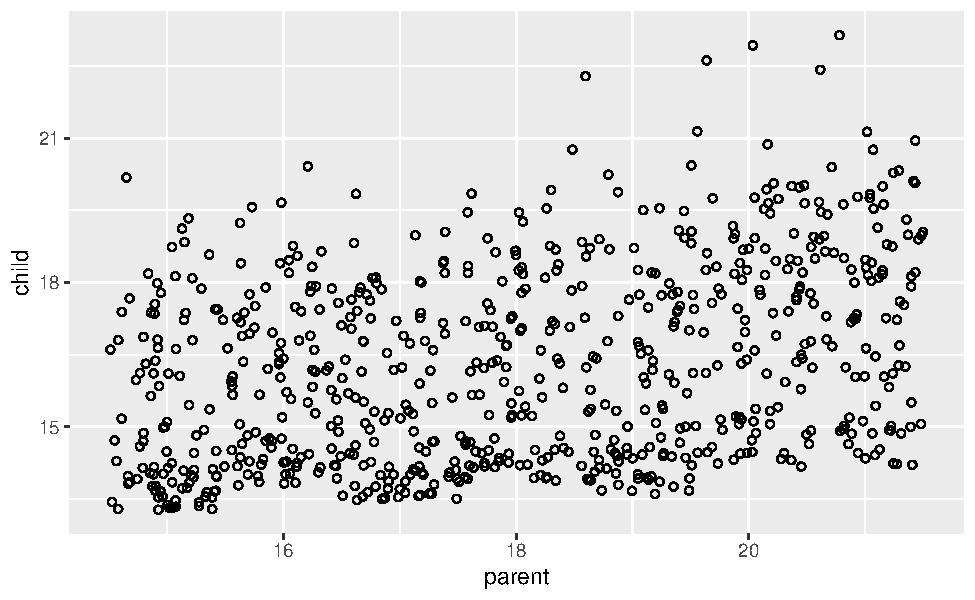
\includegraphics{01_Lecture_Notes_files/figure-latex/peas-scatter-1.pdf}

\begin{enumerate}
\def\labelenumi{\arabic{enumi}.}
\item
  Describe the scatterplot. \vspace{2in}
\item
  Draw a line that best fits these data.
\item
  Describe your reasoning to have drawn that particular line.
  \vspace{1in}
\end{enumerate}

\newpage

\hypertarget{scatterplot-of-parent-seed-diameter-mm-and-child-seed-diameter-mm---version-2}{%
\subsection{2. Scatterplot of Parent Seed Diameter (mm) and Child Seed
Diameter (mm) - Version
2}\label{scatterplot-of-parent-seed-diameter-mm-and-child-seed-diameter-mm---version-2}}

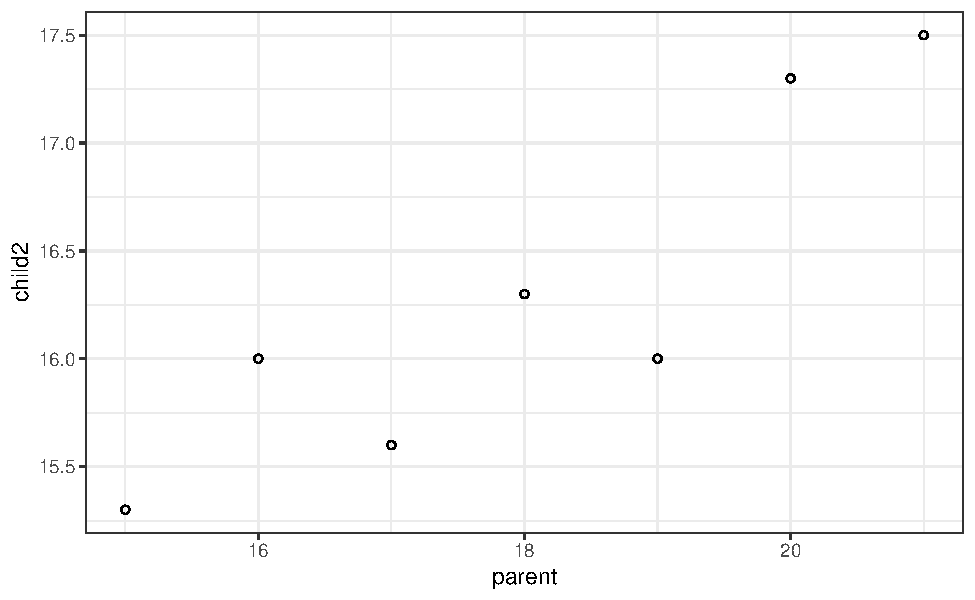
\includegraphics{01_Lecture_Notes_files/figure-latex/peas-scatter-adj-1.pdf}

\begin{enumerate}
\def\labelenumi{\arabic{enumi}.}
\item
  Describe the scatterplot. \vspace{2in}
\item
  Draw a line that best fits these data.
\item
  Describe your reasoning to have drawn that particular line.
  \vspace{1in}
\end{enumerate}

\newpage

\hypertarget{numeric-values}{%
\subsection{3. Numeric values}\label{numeric-values}}

Frank also mentions that a statistician friend ran a regression model --
you remember those from your intro statistics class! -- but isn't sure
what it means. Can you help? They show you the following equation(s)
that they have:

\[ y = \beta_0 + \beta_1Parent + \epsilon \]

\[ y= 10.114 + 0.343Parent \]

\begin{enumerate}
\def\labelenumi{\arabic{enumi}.}
\tightlist
\item
  In the second equation, what do each of the numbers mean? Please
  interpret each in a sentence for Frank.
\end{enumerate}

\vspace{1in}

\begin{enumerate}
\def\labelenumi{\arabic{enumi}.}
\tightlist
\item
  Illustrate how to use this result to make predictions. What would this
  model predict a child seed's diameter would be if the parent seed were
  16, 17 and 20mm (make a prediction for each possible parent size)?
\end{enumerate}

\vspace{2.5in}

\hypertarget{what-to-adjust-for}{%
\subsection{4. What to adjust for?}\label{what-to-adjust-for}}

Frank knows that it isn't just genetics that affect a child's
development but doesn't know how to account for that quantitatively.
You're about to take a class on mulitple regression and suggest that you
might be able to ``control for'' some of the other things that might be
associated with both child and parent seed size that could explain this
relationship. Help brainstorm with Frank what some idea are so they know
what else to measure in their data other than just seed size.

\begin{enumerate}
\def\labelenumi{\arabic{enumi}.}
\tightlist
\item
  List 2-3 other factors that are associated with child and parent seed
  diameter that could explain this relationship.
\end{enumerate}

\newpage

\end{document}
